\providecommand{\qcOne}{\mathbf{1}}   %
\providecommand{\qcTwo}{\mathbf{2}}   %
\providecommand{\qcor}[1]{\ulcorner#1\urcorner}   %

\section{箭头\trInfinityCategory}\label{sec:infinity-categories-of-arrows}

本节中，我们把 3.1 节开头的讨论复刻一遍，用任意的\trInfinityCategory{} $A$ 顶替%
\trQuasiCategory{} $Q$。上一节的分析本可以在这一般性的设定中直接展开，只是代价是%
多出一层抽象与更使人混淆的记号——此时\trFunctorSpace{} $\mathrm{Fun}(X,A)$ 取代了%
\trQuasiCategory{} $Q$。
回忆：\trInfinityCategory{}的\trElement{}定义为\trFunctor{} $a\colon\qcOne\to A$。%
同义反复地说，$A$ 的诸\trElement{}正是 $A$ 的\trUnderlyingQuasiCategory{}%
$\mathrm{Fun}(\qcOne,A)$ 的诸顶点。本节中，我们定义并研究一个\trInfinityCategory{}%
$A^{2}$，其\trElement{}恰是 $A$ 的\trUnderlyingQuasiCategory{}中的诸 1-\trSimplex{}。%
我们把 $A^{2}$ 称为 $A$ 中的\textbf{\trArrowInfinityCategory}（∞-category of arrows），并径称其%
\trElement{}为 $A$ 的\emph{箭头}（arrow）。%
事实上，这一构造我们此前早已默认引入过。回忆：$\qcTwo$ 是我们对\trQuasiCategory{}%
$\Delta[1]$ 的惯用记号，它即\trCategory{} $2$——带唯一一条非恒同态射 $0\to 1$ 的%
那个——的\trNerve{}。

\begin{definition}[\trArrowInfinityCategory]\label{def:arrow-infinity-category}
设 $A$ 为一个\trInfinityCategory。$A$ 中的\trArrowInfinityCategory{}是单纯\trCotensor{}
$A^{\qcTwo}$ 连同由包含 $\partial\Delta[1]\hookrightarrow\Delta[1]$ 诱导的典范%
\trEndpointEvaluation{}等价纤维化
\[
A^{\qcTwo}\coloneqq A^{\Delta[1]}\xrightarrow[\ (p_{1},p_{0})\ ]{A^{\partial\Delta[1]}\cong A\times A}
\]
为简洁起见，我们把由包含 $0\colon\qcOne\hookrightarrow\qcTwo$ 诱导的%
\trDomainEvaluation{}记作 $p_{0}\colon A^{\qcTwo}\twoheadrightarrow A$，
把由 $1\colon\qcOne\hookrightarrow\qcTwo$ 诱导的\trCodomainEvaluation{}记作%
$p_{1}\colon A^{\qcTwo}\twoheadrightarrow A$。
\end{definition}

作为\trHomotopyTwoCategory{}中的一个对象，\trArrowInfinityCategory{}配备有一个典范 2-\trCell{}，%
我们现在就来构造它。

\begin{lemma}[\trGenericArrow]\label{lem:generic-arrow}
对任意\trInfinityCategory{} $A$，\trArrowInfinityCategory $A^{2}$ 配备有一个典范 2-\trCell
\begin{rveq}\label{eq:generic-arrow}
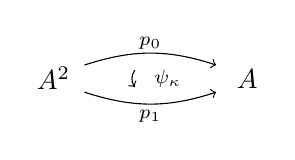
\begin{tikzpicture}[x=1.4em,y=1.4em,baseline=(current bounding box.center)]
  \node (a) at (0,0) {$A^{2}$};
  \node (b) at (5,0) {$A$};
  \draw[->] (0.8,0.35) to[bend left=18] (4.2,0.35);
  \node at (2.5,0.92) {$\scriptstyle p_{0}$};
  \draw[->] (0.8,-0.35) to[bend right=18] (4.2,-0.35);
  \node at (2.5,-0.97) {$\scriptstyle p_{1}$};
  \draw[->] (2.1,0.22) to[bend right=35] (2.1,-0.22);
  \node at (2.95,0.0) {$\scriptstyle\psi_{\kappa}$};
\end{tikzpicture}
\end{rveq}
我们称之为以 $A$ 为余定义域的\textbf{\trGenericArrow}（generic arrow）。
\end{lemma}

\begin{proof}
\trSimplicial\trCotensor{}具有题外话 1.2.6 所描述的严格\trUniversalProperty{}：%
也就是说，$A^{2}$ 由自然同构
\begin{rveq}\label{eq:fun-cotensor-iso}
\mathrm{Fun}(X,A^{2})\cong\mathrm{Fun}(X,A)^{2}
\end{rveq}
所刻画。由\trYonedaLemma{}，自然同构 \eqref{eq:fun-cotensor-iso} 的数据被其%
「\trGenericElement」所编码——后者定义为恒同在表示对象处的像。%
这里，恒同函子 $\mathrm{id}\colon A^{2}\to A^{2}$ 被映为 $\mathrm{Fun}(A^{2},A)^{2}$%
的一个\trElement——亦即 $\mathrm{Fun}(A^{2},A)$ 中的一个 1-\trSimplex——由引理%
1.4.3，它表示\trHomotopyTwoCategory{}中的一个 2-\trCell{} $\kappa$。
要看清 $\kappa$ 的源与靶必是\trDomainEvaluation{}与\trCodomainEvaluation{}这两个函子——二者由对端点%
包含 $\qcOne+\qcOne\hookrightarrow\qcTwo$ 作余张量而定义——
我们利用自然同构 \eqref{eq:fun-cotensor-iso} 在余张量变元上的自然性：
\begin{center}
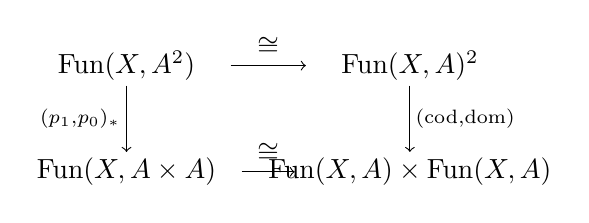
\begin{tikzpicture}[x=1.6em,y=1.6em]
  \node (tl) at (0,1.2) {$\mathrm{Fun}(X,A^{2})$};
  \node (tr) at (6.4,1.2) {$\mathrm{Fun}(X,A)^{2}$};
  \node (bl) at (0,-1.2) {$\mathrm{Fun}(X,A\times A)$};
  \node (br) at (6.4,-1.2) {$\mathrm{Fun}(X,A)\times\mathrm{Fun}(X,A)$};
  \draw[->] (2.35,1.2) -- node[above]{$\cong$} (4.05,1.2);
  \draw[->] (2.6,-1.2) -- node[above]{$\cong$} (3.8,-1.2);
  \draw[->] (0,0.75) -- (0,-0.75);
  \node at (-1.05,0) {$\scriptstyle(p_{1},p_{0})_{*}$};
  \draw[->] (6.4,0.75) -- (6.4,-0.75);
  \node at (7.65,0) {$\scriptstyle(\mathrm{cod},\mathrm{dom})$};
\end{tikzpicture}
\end{center}
恒同函子沿右上复合被映到函子对 $(\mathrm{cod}\,\kappa,\mathrm{dom}\,\kappa)$，而沿%
左下复合被映到函子对 $(p_{1},p_{0})$。
\end{proof}

存在一个与\cref{def:arrow-infinity-category}相类比的 2-范畴论\trLimit{}概念：它对%
任意对象 $A$ 构造以 $A$ 为余定义域的泛 2-\trCell——亦即与 1-\trCategory{} $2$ 作的%
（范畴论的）\trCotensor{}。其\trUniversalProperty{}与 \eqref{eq:fun-cotensor-iso}%
相类似，只是以该 2-\trCategory{}的 \trHomCategory{}顶替\trFunctorSpace{}（见定义 A.4.1）。%
在\trCategory{}的 2-\trCategory{}中，2-\trCotensor{}定义了\trCategoryOfArrows{}。
在\trHomotopyTwoCategory{}中，再次由\trYonedaLemma{}，数据 \eqref{eq:generic-arrow}%
编码了\trCategory{}之间的一个\trNaturalTransformation
\[
\mathrm{hFun}(X,A^{2})\longrightarrow\mathrm{hFun}(X,A)^{2}
\]
但它并\emph{不是}自然同构，甚至连\trCategory{}之间的自然等价也不是。不过，它确实%
赋予\trArrowInfinityCategory{}一条如下形式的「弱」\trUniversalProperty{}：

\begin{proposition}[\trArrowInfinityCategory{}的弱泛性质]\label{prop:weak-universal-property}
以 $A$ 为余定义域的\trGenericArrow \eqref{eq:generic-arrow} 在\trHomotopyTwoCategory{}中%
具有由下述三种运算给出的弱\trUniversalProperty{}：
\begin{enumerate}[label=(\roman*)]
\item \textbf{1-\trCell{}归纳：}%
给定 $A$ 上的一项\trNaturalTransformation{}，如下左图所示：
\begin{center}
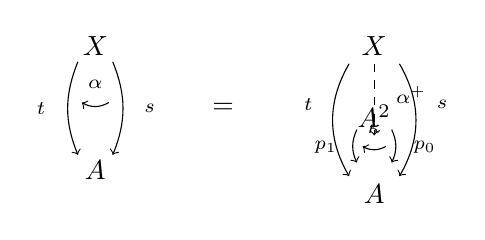
\begin{tikzpicture}[x=1.4em,y=1.4em]
  \node (Xl) at (0,1.6) {$X$};
  \node (Al) at (0,-1.6) {$A$};
  \draw[->] (-0.45,1.2) to[bend right=22] (-0.45,-1.2);
  \node at (-1.4,0) {$\scriptstyle t$};
  \draw[->] (0.45,1.2) to[bend left=22] (0.45,-1.2);
  \node at (1.4,0) {$\scriptstyle s$};
  \draw[->] (0.35,0.15) to[bend left=30] (-0.35,0.15);
  \node at (0,0.62) {$\scriptstyle\alpha$};
  \node at (3.3,0) {$=$};
  \node (Xr) at (7.2,1.6) {$X$};
  \node (M) at (7.2,-0.2) {$A^{2}$};
  \node (Ar) at (7.2,-2.2) {$A$};
  \draw[->,dashed] (7.2,1.15) -- (7.2,-0.7);
  \node at (8.15,0.35) {$\scriptstyle\ulcorner\alpha^{+}\urcorner$};
  \draw[->] (6.55,1.15) to[bend right=30] (6.55,-1.75);
  \node at (5.5,0.1) {$\scriptstyle t$};
  \draw[->] (7.85,1.15) to[bend left=30] (7.85,-1.75);
  \node at (8.95,0.1) {$\scriptstyle s$};
  \draw[->] (6.75,-0.55) to[bend right=25] (6.75,-1.4);
  \node at (5.95,-1.0) {$\scriptstyle p_{1}$};
  \draw[->] (7.65,-0.55) to[bend left=25] (7.65,-1.4);
  \node at (8.5,-1.0) {$\scriptstyle p_{0}$};
  \draw[->] (7.5,-0.98) to[bend left=30] (6.9,-0.98);
  \node at (7.2,-0.55) {$\scriptstyle\kappa$};
\end{tikzpicture}
\end{center}
则存在\trFunctor{} $\qcor{\alpha^{+}}\colon X\to A^{2}$，使得 $s=p_{0}\qcor{\alpha^{+}}$、%
$t=p_{1}\qcor{\alpha^{+}}$，且 $\alpha=\kappa\qcor{\alpha^{+}}$。
\item \textbf{2-\trCell{}归纳：}%
给定\trFunctor{} $a,a'\colon X\to A^{2}$ 与\trNaturalTransformation{} $\tau_{1}$、%
$\tau_{0}$，使得
\begin{center}
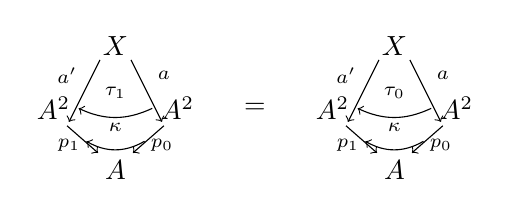
\begin{tikzpicture}[x=1.4em,y=1.4em]
  \node (X) at (0,1.5) {$X$};
  \node (Ml) at (-1.6,-0.1) {$A^{2}$};
  \node (Mr) at (1.6,-0.1) {$A^{2}$};
  \node (A) at (0,-1.7) {$A$};
  \draw[->] (-0.4,1.15) -- (-1.2,-0.45);
  \node at (-1.25,0.75) {$\scriptstyle a'$};
  \draw[->] (0.4,1.15) -- (1.2,-0.45);
  \node at (1.25,0.75) {$\scriptstyle a$};
  \draw[->] (0.95,-0.1) to[bend left=25] (-0.95,-0.1);
  \node at (0,0.3) {$\scriptstyle\tau_{1}$};
  \draw[->] (-1.25,-0.55) -- (-0.45,-1.25);
  \node at (-1.2,-1.05) {$\scriptstyle p_{1}$};
  \draw[->] (1.25,-0.55) -- (0.45,-1.25);
  \node at (1.2,-1.05) {$\scriptstyle p_{0}$};
  \draw[->] (0.75,-0.95) to[bend left=30] (-0.75,-0.95);
  \node at (0,-0.58) {$\scriptstyle\kappa$};
  \node at (3.6,-0.1) {$=$};
  \begin{scope}[shift={(7.2,0)}]
  \node (X) at (0,1.5) {$X$};
  \node (Ml) at (-1.6,-0.1) {$A^{2}$};
  \node (Mr) at (1.6,-0.1) {$A^{2}$};
  \node (A) at (0,-1.7) {$A$};
  \draw[->] (-0.4,1.15) -- (-1.2,-0.45);
  \node at (-1.25,0.75) {$\scriptstyle a'$};
  \draw[->] (0.4,1.15) -- (1.2,-0.45);
  \node at (1.25,0.75) {$\scriptstyle a$};
  \draw[->] (0.95,-0.1) to[bend left=25] (-0.95,-0.1);
  \node at (0,0.3) {$\scriptstyle\tau_{0}$};
  \draw[->] (-1.25,-0.55) -- (-0.45,-1.25);
  \node at (-1.2,-1.05) {$\scriptstyle p_{1}$};
  \draw[->] (1.25,-0.55) -- (0.45,-1.25);
  \node at (1.2,-1.05) {$\scriptstyle p_{0}$};
  \draw[->] (0.75,-0.95) to[bend left=30] (-0.75,-0.95);
  \node at (0,-0.58) {$\scriptstyle\kappa$};
  \end{scope}
\end{tikzpicture}
\end{center}
则存在\trNaturalTransformation{} $\tau\colon a\Rightarrow a'$，使得 $p_{1}\tau=\tau_{1}$%
且 $p_{0}\tau=\tau_{0}$。
\item \textbf{2-\trCell{}保守性：}%
对任何\trNaturalTransformation
\begin{center}
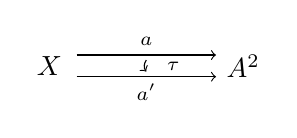
\begin{tikzpicture}[x=1.4em,y=1.4em]
  \node (X) at (0,0) {$X$};
  \node (M) at (5,0) {$A^{2}$};
  \draw[->] (0.7,0.28) -- (4.3,0.28);
  \node at (2.5,0.64) {$\scriptstyle a$};
  \draw[->] (0.7,-0.28) -- (4.3,-0.28);
  \node at (2.5,-0.68) {$\scriptstyle a'$};
  \draw[->] (2.5,0.15) to[bend right=35] (2.5,-0.15);
  \node at (3.2,0.0) {$\scriptstyle\tau$};
\end{tikzpicture}
\end{center}
若 $p_{1}\tau$ 与 $p_{0}\tau$ 皆为\trIsomorphism{}，则 $\tau$ 是\trIsomorphism{}。
\end{enumerate}
\end{proposition}

\begin{proof}
令 $Q=\mathrm{Fun}(X,A)$ 并应用引理 3.1.1，可见 \trHomCategory{}之间的自然映射
\begin{center}
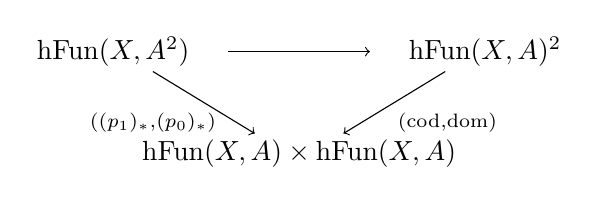
\begin{tikzpicture}[x=1.6em,y=1.6em]
  \node (tl) at (0,1.3) {$\mathrm{hFun}(X,A^{2})$};
  \node (tr) at (8.4,1.3) {$\mathrm{hFun}(X,A)^{2}$};
  \node (bm) at (4.2,-1.0) {$\mathrm{hFun}(X,A)\times\mathrm{hFun}(X,A)$};
  \draw[->] (2.6,1.3) -- (5.8,1.3);
  \draw[->] (0.9,0.85) -- (3.2,-0.55);
  \node at (0.9,-0.3) {$\scriptstyle((p_{1})_{*},(p_{0})_{*})$};
  \draw[->] (7.5,0.85) -- (5.2,-0.55);
  \node at (7.55,-0.3) {$\scriptstyle(\mathrm{cod},\mathrm{dom})$};
\end{tikzpicture}
\end{center}
——它居于 $\mathrm{hFun}(X,A\times A)\cong\mathrm{hFun}(X,A)\times\mathrm{hFun}(X,A)$%
之上——是一个\trSmotheringFunctor{}。对象上的满射性由 1-\trCell{}归纳表达，满性由%
2-\trCell{}归纳表达，而保守性由 2-\trCell{}保守性表达。
\end{proof}

注意，表示一个给定的\trNaturalTransformation{} $\alpha$（以 $X$ 为定义域、以 $A$ 为%
余定义域）的诸\trFunctor{} $\qcor{\alpha^{+}}\colon X\to A^{2}$ 并不唯一。然而，它们在%
「纤维化」同构之下唯一——这类同构与 $(p_{1},p_{0})\colon A^{2}\twoheadrightarrow A\times A$%
作\trWhiskering{}后成为恒同：%

\begin{proposition}\label{prop:whiskering-bijection}
与 \eqref{eq:generic-arrow} 的\trWhiskering{}在如下左所示的、以 $X$ 为定义域且以 $A$ 为%
余定义域的诸\trNaturalTransformation{}，与如下右所示的、诸\trFunctor{} $X\to A^{2}$ 的%
\trFiberedIsomorphism{}类之间诱导出一个双射：
\[
\left\{\vcenter{\hbox{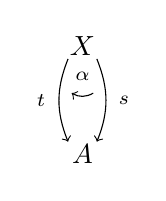
\begin{tikzpicture}[x=1.3em,y=1.3em]
  \node (X) at (0,1.5) {$X$};
  \node (A) at (0,-1.5) {$A$};
  \draw[->] (-0.4,1.15) to[bend right=22] (-0.4,-1.15);
  \node at (-1.15,0) {$\scriptstyle t$};
  \draw[->] (0.4,1.15) to[bend left=22] (0.4,-1.15);
  \node at (1.15,0) {$\scriptstyle s$};
  \draw[->] (0.3,0.2) to[bend left=30] (-0.3,0.2);
  \node at (0,0.66) {$\scriptstyle\alpha$};
\end{tikzpicture}}}\right\}
\;\longleftrightarrow\;
\left\{\vcenter{\hbox{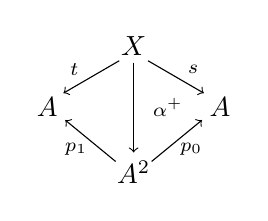
\begin{tikzpicture}[x=1.3em,y=1.3em]
  \node (X) at (0,1.6) {$X$};
  \node (Al) at (-2.4,-0.1) {$A$};
  \node (Ar) at (2.4,-0.1) {$A$};
  \node (M) at (0,-1.9) {$A^{2}$};
  \draw[->] (-0.4,1.2) -- (-1.95,0.3);
  \node at (-1.65,0.95) {$\scriptstyle t$};
  \draw[->] (0.4,1.2) -- (1.95,0.3);
  \node at (1.65,0.95) {$\scriptstyle s$};
  \draw[->] (0,1.15) -- (0,-1.35);
  \node at (0.95,-0.1) {$\scriptstyle\ulcorner\alpha^{+}\urcorner$};
  \draw[->] (-0.5,-1.6) -- (-1.9,-0.45);
  \node at (-1.6,-1.25) {$\scriptstyle p_{1}$};
  \draw[->] (0.5,-1.6) -- (1.9,-0.45);
  \node at (1.6,-1.25) {$\scriptstyle p_{0}$};
\end{tikzpicture}}}\right\}_{/\cong}
\]
其中诸\trFiberedIsomorphism{}由可逆 2-\trCell
\begin{center}
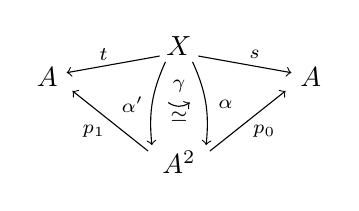
\begin{tikzpicture}[x=1.4em,y=1.4em]
  \node (X) at (0,1.7) {$X$};
  \node (Al) at (-3.4,0.9) {$A$};
  \node (Ar) at (3.4,0.9) {$A$};
  \node (M) at (0,-1.3) {$A^{2}$};
  \draw[->] (-0.5,1.45) -- (-2.9,1.02);
  \node at (-1.95,1.5) {$\scriptstyle t$};
  \draw[->] (0.5,1.45) -- (2.9,1.02);
  \node at (1.95,1.5) {$\scriptstyle s$};
  \draw[->] (-0.35,1.3) to[bend right=15] (-0.7,-0.85);
  \node at (-1.2,0.2) {$\scriptstyle\ulcorner\alpha'\urcorner$};
  \draw[->] (0.35,1.3) to[bend left=15] (0.7,-0.85);
  \node at (1.2,0.2) {$\scriptstyle\ulcorner\alpha\urcorner$};
  \draw[->] (-0.28,0.25) to[bend right=35] (0.28,0.25);
  \node at (0,0.68) {$\scriptstyle\gamma$};
  \node at (0,-0.12) {$\scriptstyle\simeq$};
  \draw[->] (-0.8,-1.0) -- (-2.75,0.55);
  \node at (-2.2,-0.5) {$\scriptstyle p_{1}$};
  \draw[->] (0.8,-1.0) -- (2.75,0.55);
  \node at (2.2,-0.5) {$\scriptstyle p_{0}$};
\end{tikzpicture}
\end{center}
给出，满足 $p_{1}\gamma=\mathrm{id}_{t}$ 与 $p_{0}\gamma=\mathrm{id}_{s}$。
\end{proposition}

\begin{proof}
引理 3.1.3 证明了\cref{prop:weak-universal-property}的\trSmotheringFunctor{}之诸%
\trFiber{}都是连通\trGroupoid{}。
$\alpha$ 之上的\trFiber{}，其对象是经\trGenericArrow $\kappa$\trWhiskering{}后给出 $\alpha$ 的%
那些\trFunctor{} $X\to A^{2}$，其态射是经 $(p_{1},p_{0})\colon A^{2}\twoheadrightarrow A\times A$%
\trWhiskering{}后成为恒同 2-\trCell{} $(\mathrm{id}_{t},\mathrm{id}_{s})$ 的那些%
\trInvertible{} 2-\trCell{}。\trSmotheringFunctor{}的作用在其余域的对象与各自的%
\trFiber{}之间定义了一个双射。
\end{proof}

我们最后一项任务是观察到：\cref{prop:weak-universal-property}的\trUniversalProperty{}%
同样为任何对象 $(e_{1},e_{0})\colon E\twoheadrightarrow A\times A$ 所享有——只要它在%
$A\times A$ 上的\trSliceInfinityCosmos{}中等价于\trArrowInfinityCategory \allowbreak$(p_{1},p_{0})\colon A^{2}\twoheadrightarrow A\times A$。%
我们有一套专门的术语，可用以简洁表达我们所想的那类\trEquivalence{}。

\begin{definition}[\trFiberedEquivalence]\label{def:fibered-equivalence}
\trInfinityCosmos{} $\mathcal{K}$ 中、在\trInfinityCategory{} $B$ 上的一条%
\textbf{\trFiberedEquivalence}（fibered equivalence）是\trSliceInfinityCosmos $\mathcal{K}_{/B}$ 中形如下式的%
一个\trEquivalence
\begin{rveq}\label{eq:fibered-equivalence}
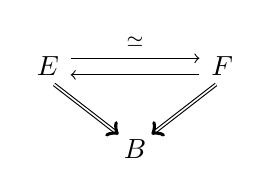
\begin{tikzpicture}[x=1.5em,y=1.5em,baseline=(current bounding box.center)]
  \node (E) at (0,0.9) {$E$};
  \node (F) at (4.2,0.9) {$F$};
  \node (B) at (2.1,-1.1) {$B$};
  \draw[->] (0.55,1.08) -- (3.65,1.08);
  \node at (2.1,1.48) {$\scriptstyle\simeq$};
  \draw[->] (3.65,0.68) -- (0.55,0.68);
  \draw[double,->] (0.15,0.45) -- (1.7,-0.75);
  \draw[double,->] (4.05,0.45) -- (2.5,-0.75);
\end{tikzpicture}
\end{rveq}
我们记 $E\simeq_{B}F$，以指明带这些定义域的指定诸等价纤维化\emph{在} $B$ \emph{上}%
等价。
\end{definition}

由命题 1.2.22(vii)，\trFiberedEquivalence{}无非是公共底上的一对等价纤维化之间的、在底%
\trInfinityCosmos{}中构成\trEquivalence{}的一个映射：遗忘函子 $\mathcal{K}_{/B}\to\mathcal{K}$%
保持且反射诸\trEquivalence{}。
然而请注意，它并不创造它们：两个\trInfinityCategory{} $E$ 与 $F$ 完全可能相互等价，%
却不存在任何与指定等价纤维化对 $E\twoheadrightarrow B$、$F\twoheadrightarrow B$%
相容的\trEquivalence{}。

\begin{warning}\label{war:fibered-equivalence-presentation}
至此，关于在\trInfinityCosmos{} $\mathcal{K}_{/B}$ 中呈现一条\trFiberedEquivalence{}所需的 2-范畴论%
数据为何，尚存某种含混；这与练习 1.4.vii 就 2-范畴 $\mathrm{h}(\mathcal{K}_{/B})$ 与%
$(\mathrm{h}\mathcal{K})_{/B}$ 之间的关系所提出的问题是相关的。
但由于命题 1.2.22(vii) 告诉我们，$\mathrm{h}\mathcal{K}$ 中单单一个涉及形如%
\eqref{eq:fibered-equivalence} 之\trFunctor{}的\trEquivalence{}便已足以保证这项目前%
尚未指明的 2-范畴论数据存在，故我们把这个问题的细致分析推迟到命题 3.6.4。
\end{warning}

\begin{proposition}[\trArrowInfinityCategory{}的唯一性]\label{prop:arrow-category-uniqueness}
对任何\trFiberedEquivalence{}于 $(p_{1},p_{0})\colon A^{2}\twoheadrightarrow A\times A$ 的%
等价纤维化 $(e_{1},e_{0})\colon E\twoheadrightarrow A\times A$，由\trEquivalence{}%
$e\colon E\rightleftarrows A^{2}$ 所编码的 2-\trCell
\begin{center}
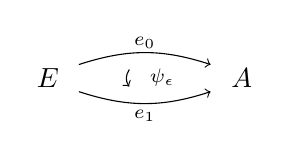
\begin{tikzpicture}[x=1.4em,y=1.4em]
  \node (a) at (0,0) {$E$};
  \node (b) at (5,0) {$A$};
  \draw[->] (0.8,0.35) to[bend left=18] (4.2,0.35);
  \node at (2.5,0.92) {$\scriptstyle e_{0}$};
  \draw[->] (0.8,-0.35) to[bend right=18] (4.2,-0.35);
  \node at (2.5,-0.97) {$\scriptstyle e_{1}$};
  \draw[->] (2.1,0.22) to[bend right=35] (2.1,-0.22);
  \node at (2.95,0.0) {$\scriptstyle\psi_{\epsilon}$};
\end{tikzpicture}
\end{center}
满足\cref{prop:weak-universal-property}的弱\trUniversalProperty{}。反之，若等价纤维化%
$(d_{1},d_{0})\colon D\twoheadrightarrow A\times A$ 与 $(e_{1},e_{0})\colon E\twoheadrightarrow A\times A$%
配备有 2-\trCell
\begin{center}
\begin{tikzpicture}[x=1.4em,y=1.4em]
  \node (a) at (0,0) {$D$};
  \node (b) at (5,0) {$A$};
  \draw[->] (0.8,0.35) to[bend left=18] (4.2,0.35);
  \node at (2.5,0.92) {$\scriptstyle d_{0}$};
  \draw[->] (0.8,-0.35) to[bend right=18] (4.2,-0.35);
  \node at (2.5,-0.97) {$\scriptstyle d_{1}$};
  \draw[->] (2.1,0.22) to[bend right=35] (2.1,-0.22);
  \node at (2.95,0.0) {$\scriptstyle\psi_{\delta}$};
  \node at (8.6,0) {与};
  \begin{scope}[shift={(12.2,0)}]
  \node (a) at (0,0) {$E$};
  \node (b) at (5,0) {$A$};
  \draw[->] (0.8,0.35) to[bend left=18] (4.2,0.35);
  \node at (2.5,0.92) {$\scriptstyle e_{0}$};
  \draw[->] (0.8,-0.35) to[bend right=18] (4.2,-0.35);
  \node at (2.5,-0.97) {$\scriptstyle e_{1}$};
  \draw[->] (2.1,0.22) to[bend right=35] (2.1,-0.22);
  \node at (2.95,0.0) {$\scriptstyle\psi_{\epsilon}$};
  \end{scope}
\end{tikzpicture}
\end{center}
且它们满足\cref{prop:weak-universal-property}的弱\trUniversalProperty{}，则%
$D\simeq_{A\times A}E$。
\end{proposition}

\begin{proof}
我们证明第一个陈述。由 1-\trCell{}归纳的定义等式 $\epsilon=\kappa e$，其中 $\kappa$ 是%
\trGenericArrow \eqref{eq:generic-arrow}。于是，与 $\epsilon$ 作粘贴所诱导的\trFunctor{}分解为%
一个复合
\begin{center}
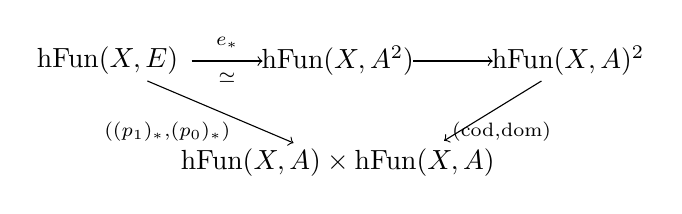
\begin{tikzpicture}[x=1.6em,y=1.6em]
  \node (l) at (0,1.3) {$\mathrm{hFun}(X,E)$};
  \node (m) at (5.2,1.3) {$\mathrm{hFun}(X,A^{2})$};
  \node (r) at (10.4,1.3) {$\mathrm{hFun}(X,A)^{2}$};
  \node (bm) at (5.2,-1.0) {$\mathrm{hFun}(X,A)\times\mathrm{hFun}(X,A)$};
  \draw[->] (1.9,1.3) -- (3.5,1.3);
  \node at (2.7,1.72) {$\scriptstyle e_{*}$};
  \node at (2.7,0.92) {$\scriptstyle\simeq$};
  \draw[->] (6.9,1.3) -- (8.7,1.3);
  \draw[->] (0.9,0.85) -- (4.2,-0.55);
  \node at (1.35,-0.3) {$\scriptstyle((p_{1})_{*},(p_{0})_{*})$};
  \draw[->] (9.8,0.85) -- (7.6,-0.5);
  \node at (8.9,-0.3) {$\scriptstyle(\mathrm{cod},\mathrm{dom})$};
\end{tikzpicture}
\end{center}
而我们的任务是证明该复合\trFunctor{}是\trSmothering{}。第一个\trFunctor{}由与%
\trEquivalence{} $e\colon E\rightleftarrows A^{2}$ 作后复合定义，是\trCategory{}之间的%
一个\trEquivalence{}；第二个\trFunctor{}则是\trSmothering{}。于是，该复合显然\trFull{}且%
\trConservative{}。为见它也对象上满，先注意由 1-\trCell{}归纳，任何 2-\trCell
\begin{center}
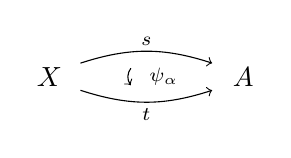
\begin{tikzpicture}[x=1.4em,y=1.4em]
  \node (a) at (0,0) {$X$};
  \node (b) at (5,0) {$A$};
  \draw[->] (0.8,0.35) to[bend left=18] (4.2,0.35);
  \node at (2.5,0.92) {$\scriptstyle s$};
  \draw[->] (0.8,-0.35) to[bend right=18] (4.2,-0.35);
  \node at (2.5,-0.97) {$\scriptstyle t$};
  \draw[->] (2.1,0.22) to[bend right=35] (2.1,-0.22);
  \node at (2.95,0.0) {$\scriptstyle\psi_{\alpha}$};
\end{tikzpicture}
\end{center}
都由 $A\times A$ 之上的某个\trFunctor{} $\qcor{\alpha^{+}}\colon X\to A^{2}$ 所表示。%
与 $e$ 的任一\trFiberedInverseEquivalence $e'$ 作复合，便给出\trFunctor
\begin{center}
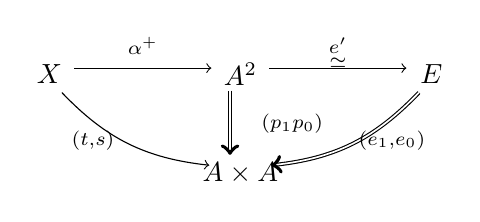
\begin{tikzpicture}[x=1.5em,y=1.5em]
  \node (X) at (0,0) {$X$};
  \node (M) at (4.6,0) {$A^{2}$};
  \node (E) at (9.2,0) {$E$};
  \node (B) at (4.6,-2.4) {$A\times A$};
  \draw[->] (0.6,0.14) -- (3.9,0.14);
  \node at (2.25,0.68) {$\scriptstyle\ulcorner\alpha^{+}\urcorner$};
  \draw[->] (5.3,0.14) -- (8.6,0.14);
  \node at (6.95,0.68) {$\scriptstyle e'$};
  \node at (6.95,0.26) {$\scriptstyle\simeq$};
  \draw[double,->] (4.35,-0.4) -- (4.35,-1.95);
  \node at (5.85,-1.2) {$\scriptstyle(p_{1}p_{0})$};
  \draw[->] (0.3,-0.45) to[bend right=20] (3.85,-2.2);
  \node at (1.05,-1.6) {$\scriptstyle(t,s)$};
  \draw[double,->] (8.9,-0.45) to[bend left=20] (5.35,-2.2);
  \node at (8.25,-1.6) {$\scriptstyle(e_{1},e_{0})$};
\end{tikzpicture}
\end{center}
其在与 $e$ 作\trPostComposition{}之后的像，与 $A\times A$ 之上的 $\qcor{\alpha^{+}}$%
\trFiberedIsomorphism{}。由于这一同构在\cref{prop:whiskering-bijection}的意义下是\trFibered{}，%
$e'\qcor{\alpha^{+}}$ 在\trFunctor{} $\mathrm{hFun}(X,E)\to\mathrm{hFun}(X,A)^{2}$ 之下的%
像便还原出 2-\trCell{} $\alpha$。这便证明了该映射对象上满，从而如所宣称的那样定义了%
一个\trSmotheringFunctor{}。反方向则留作\cref{ex:converse-of-uniqueness}，并将在更一般的%
语境中于命题 3.4.11 得证。
\end{proof}

\begin{convention}\label{conv:arrow-infinity-category-appellation}
由于\cref{prop:arrow-category-uniqueness}，我们把「\trArrowInfinityCategory」这一称谓从%
\cref{def:arrow-infinity-category}所构造的严格模型扩充到任何\trFiberedEquivalence{}于它的%
\trInfinityCategory{}。
\end{convention}

经\cref{lem:smothering-free}，本节的结果可扩充为：\trInfinityCategory{} $A$ 与\trFreeCategory{} $J$ 之%
余张量 $A^{J}$ 的相应弱\trUniversalProperty——邀请读者自行探索。

\subsection*{练习}

\begin{exercise}\label{ex:arrow-representations}
本练习重温\cref{prop:whiskering-bijection}的结果。
\begin{enumerate}[label=(\roman*)]
\item 证明：\trQuasiCategory{} $Q$ 中一对平行的 1-\trSimplex{} $f,g\colon x\to y$ 是%
\trHomotopic{}，当且仅当作为 $Q^{2}$ 的\trElement{}，二者经由一个沿 $(p_{1},p_{0})\colon Q^{2}\twoheadrightarrow Q\times Q$%
投影为恒同的\trIsomorphism{}而\trIsomorphism{}。
\item 由此推出：任一\trInfinityCosmos{}中两个\trInfinityCategory{} $X$ 与 $A$ 之间%
\trFunctorSpace{}里的一对平行 1-箭头表示同一\trNaturalTransformation{}，当且仅当作为%
$\mathrm{Fun}(X,A)^{2}\cong\mathrm{Fun}(X,A^{2})$ 的\trElement{}，二者经由一个定义域%
分量与余定义域分量皆为恒同的\trIsomorphism{}而\trIsomorphism{}。
\item 再由此推出：$\mathrm{Fun}(X,A)$ 中一对平行的 1-箭头——它们可编码为\trFunctor{}%
$X\to A^{2}$——表示同一\trNaturalTransformation{}，当且仅当二者由一个\trFiberedIsomorphism{}相连：%
\begin{center}
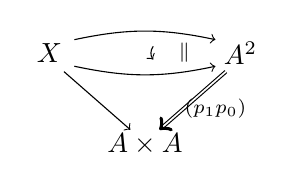
\begin{tikzpicture}[x=1.5em,y=1.5em]
  \node (X) at (0,0) {$X$};
  \node (M) at (4.6,0) {$A^{2}$};
  \node (B) at (2.3,-2.2) {$A\times A$};
  \draw[->] (0.6,0.32) to[bend left=12] (4.0,0.32);
  \draw[->] (0.6,-0.32) to[bend right=12] (4.0,-0.32);
  \draw[->] (2.5,0.16) to[bend right=35] (2.5,-0.16);
  \node at (3.25,0.0) {$\scriptstyle\parallel$};
  \draw[->] (0.35,-0.45) -- (1.95,-1.85);
  \draw[double,->] (4.25,-0.45) -- (2.65,-1.85);
  \node at (4.0,-1.35) {$\scriptstyle(p_{1}p_{0})$};
\end{tikzpicture}
\end{center}
\end{enumerate}
\end{exercise}

\begin{exercise}\label{ex:converse-of-uniqueness}
证明\cref{prop:arrow-category-uniqueness}的逆蕴含。
\end{exercise}

\begin{exercise}\label{ex:cotensor-weak-universal-property}
把\cref{prop:weak-universal-property}与\cref{prop:whiskering-bijection}的结果
推广到：由某个\trReflexiveDirectedGraph{}自由生成的\trCategory{} $J$ 的%
\trInfinityCategory{} $A$ 的余张量 $A^J$ 的弱泛性质。
\end{exercise}

